\documentclass[11pt,a4paper]{article}

\usepackage{fontspec}
\usepackage{polyglossia}
\setdefaultlanguage{french}
\setotherlanguage[variant=polytonic]{greek}

\setmainfont{FreeSerif}
\setsansfont{FreeSans}
\setmonofont{FreeMono}
\newfontfamily\greekfont{FreeSerif}
\newfontfamily\greekfontsf{FreeSans}
\newfontfamily\greekfonttt{FreeMono}

\usepackage[margin=1.8cm, top=2.1cm, bottom=2.1cm]{geometry}
\usepackage{amsmath}
\usepackage{graphicx}
\usepackage{xcolor}
\usepackage{booktabs}
\usepackage{longtable}
\usepackage{array}
\usepackage{float}
\usepackage{caption}
\usepackage{fancyhdr}
\usepackage{titlesec}
\usepackage{hyperref}

\definecolor{RavennasRed}{HTML}{6E1914}
\definecolor{RavennasBlue}{HTML}{194173}
\definecolor{ParchmentBg}{HTML}{FAF6EE}
\definecolor{BorderGold}{HTML}{9E8764}

\hypersetup{
    colorlinks=true,
    linkcolor=RavennasRed,
    urlcolor=RavennasBlue,
    citecolor=RavennasBlue,
    pdftitle={Manuel pratique et illustre de dechiffrement du Codex Ravennas 429},
    pdfauthor={Dossier Paleographique — Les Thesmophories d'Aristophane}
}

\pagestyle{fancy}
\fancyhf{}
\fancyhead[L]{\small\textit{Manuel de déchiffrement du Codex Ravennas 429 (ff. 162v--177r)}}
\fancyhead[R]{\small\textit{Aristophane, Les Thesmophories}}
\fancyfoot[C]{\thepage}
\renewcommand{\headrulewidth}{0.4pt}

\titleformat{\section}
  {\normalfont\Large\bfseries\color{RavennasRed}}{\thesection.}{0.6em}{}[\vspace{2pt}\titlerule]
\titleformat{\subsection}
  {\normalfont\large\bfseries\color{RavennasBlue}}{\thesubsection.}{0.5em}{}
\titleformat{\subsubsection}
  {\normalfont\normalsize\bfseries\color{RavennasRed}}{\thesubsubsection.}{0.5em}{}

\captionsetup{font=small, labelfont={bf,color=RavennasRed}}

\newcommand{\platefig}[3]{%
  \begin{figure}[H]
    \centering
    \fboxsep=2pt\fboxrule=0.8pt
    \fcolorbox{BorderGold}{white}{\includegraphics[width=0.97\textwidth,height=0.80\textheight,keepaspectratio]{exemples_dechiffrement/#1}}
    \caption{#2}
    \label{#3}
  \end{figure}
}

\begin{document}

\begin{titlepage}
    \centering
    \vspace*{1.2cm}
    {\scshape\Large Dossier Paléographique, Codicologique et Philologique\par}
    \vspace{0.8cm}
    \rule{\textwidth}{1.5pt}\\[0.5cm]
    {\huge\bfseries\color{RavennasRed} Manuel pratique et illustré de déchiffrement\\du \textit{Codex Ravennas 429}\par}
    \vspace{0.4cm}
    {\Large\itshape\color{RavennasBlue} Apprendre à lire l'écriture byzantine des \textit{Thesmophories} d'Aristophane\\(Ravenne, Biblioteca Classense, Ms. 429, ff. 162v--177r)\par}
    \vspace{0.4cm}
    \rule{\textwidth}{1.5pt}\\[1.0cm]

    \fboxsep=3pt\fboxrule=1pt
    \fcolorbox{BorderGold}{white}{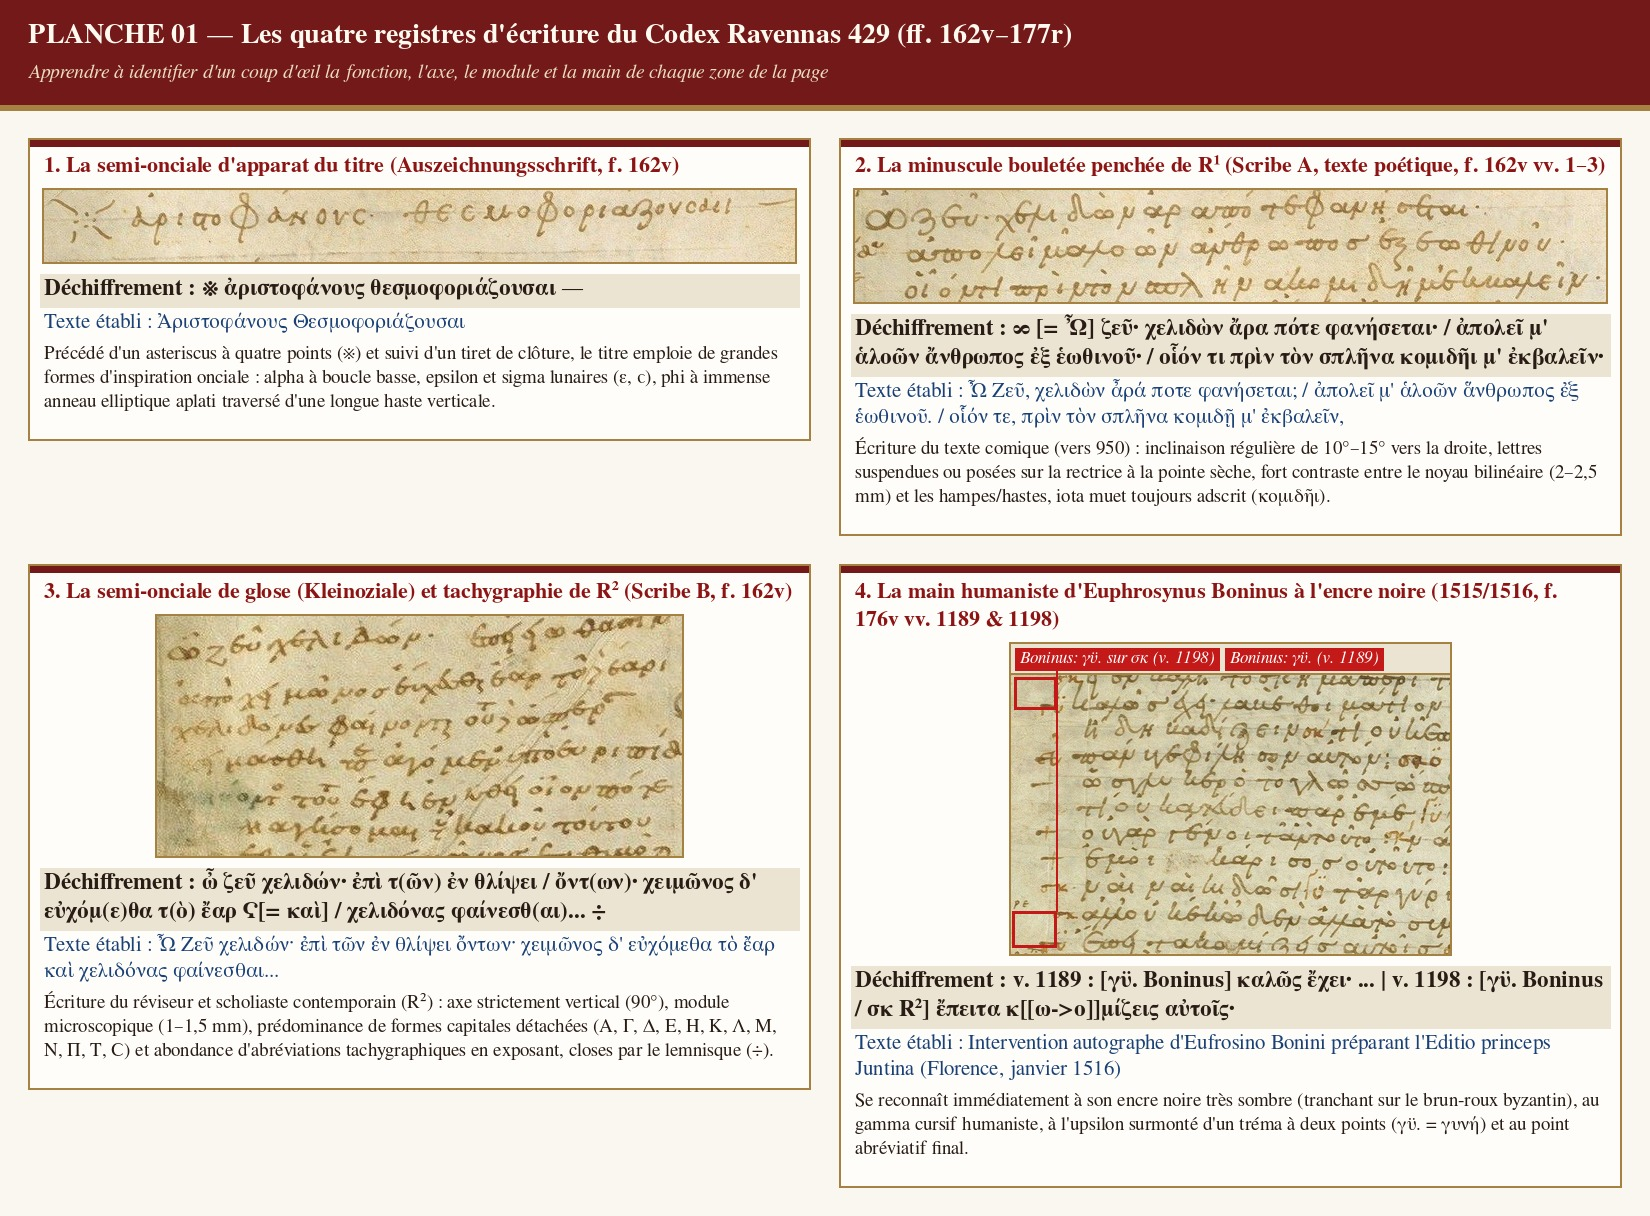
\includegraphics[width=0.86\textwidth]{exemples_dechiffrement/01_les_quatre_registres_ecriture_ravennas.jpg}}

    \vfill
    {\normalsize
    \textbf{Contenu pédagogique du manuel :}\\
    Abécédaire photographique complet des 24 lettres ($\text{R}^1$ et $\text{R}^2$) $\cdot$ Les 6 grands pièges de lecture (« faux-amis »)\\
    Dictionnaire visuel des ligatures ($\varepsilon$-, $\sigma$-, $\pi\rho$, $\tau\rho$, $-\lambda\lambda-$) $\cdot$ Règle de l'iota muet adscrit et ponctuation dramatique\\
    Monogrammes de personnages (\textit{notae personarum}), tachygraphie des scholies ($\Sigma^{\text{R}}$) et \textit{parepigraphai} antiques\\
    Anatomie des grattages sur parchemin (\textit{in rasura}) $\cdot$ Parcours d'entraînement progressif en 5 niveaux (24 planches HD)\par}
    \vspace{0.6cm}
    {\large\bfseries Constantinople (env. 950--980) $\longrightarrow$ Édition critique et diplomatique\par}
\end{titlepage}

\tableofcontents
\newpage

% ==============================================================================
\section{Introduction méthodologique : comment aborder une page du \textit{Ravennas}}
% ==============================================================================

Ouvrir pour la première fois un feuillet du \textit{Codex Ravennas 429} (milieu du X\textsuperscript{e} siècle) provoque souvent chez l'helléniste habitué aux polices typographiques modernes (Didot, Porson, Gentium) un sentiment de dépaysement visuel. Certaines lettres paraissent familières, mais d'autres semblent inverser les valeurs de notre alphabet : ce qui ressemble à un \texttt{μ} moderne est en réalité un \textbf{nu} ($\nu$), ce qui ressemble à un \texttt{h} latin est un \textbf{êta} ($\eta$), et ce qui ressemble à un \texttt{u} est le plus souvent un \textbf{bêta} ($\beta$) !

Pourtant, l'écriture du \textit{Ravennas} est l'une des plus régulières, des plus harmonieuses et des plus rigoureuses de toute la calligraphie byzantine de la « Renaissance macédonienne ». Dès que l'œil possède la grille de décodage de ses tracés (\textit{ductus}) et de ses ligatures, le déchiffrement devient non seulement fluide, mais passionnant : on lit directement par-dessus l'épaule des deux copistes constantinopolitains qui nous ont sauvé \textit{Les Thesmophories}.

\subsection{Les quatre registres d'écriture présents sur un même folio (Planche 01)}

Avant de chercher à lire un mot, il faut identifier \textbf{dans quelle zone de la page} et \textbf{dans quel registre graphique} on se trouve. Une page des \textit{Thesmophories} comporte en effet \textbf{quatre registres d'écriture bien distincts}, répartis entre deux mains contemporaines :
\begin{itemize}
    \item \textbf{Le Scribe A ($\text{R}^1$)}, qui copie la colonne centrale du texte poétique d'Aristophane ;
    \item \textbf{Le Scribe B ($\text{R}^2$)}, réviseur et scholiaste du même atelier (\textit{scriptorium}), qui ajoute les titres courants, les sigles des personnages (\textit{notae personarum}), les gloses interlinéaires et les scholies marginales ($\Sigma^{\text{R}}$).
\end{itemize}

\platefig{01_les_quatre_registres_ecriture_ravennas.jpg}{Planche 01 — Les quatre registres d'écriture d'une page du \textit{Codex Ravennas 429} (f. 162v).}{fig:pl01}

\begin{table}[H]
\centering
\small
\begin{tabular}{@{}p{2.2cm}p{3.0cm}cp{3.5cm}p{5.5cm}@{}}
\toprule
\textbf{Registre} & \textbf{Emplacement} & \textbf{Main} & \textbf{Style calligraphique} & \textbf{Caractéristiques de déchiffrement} \\
\midrule
\textbf{Registre 1} & Marge supérieure ou titre initial & $\text{R}^1$/$\text{R}^2$ & Majuscule d'apparat (\textit{Auszeichnungsmajuskel}) & Lettres capitales d'inspiration épigraphique et onciale (Α, Ε, Θ, Μ, Σ, Φ), détachées sans ligatures. \\
\addlinespace
\textbf{Registre 2} & Colonne centrale (40--43 lignes/page) & $\text{R}^1$ & Minuscule livresque bouclée (\textit{Perlschrift}) & Écriture souple, suspendue sous la réglure, riche en ligatures cursives (ει, επ, στ, σπ) et en allographes mixtes. \\
\addlinespace
\textbf{Registre 3} & Marge au ras des vers & $\text{R}^2$ & Monogrammes scéniques (\textit{notae personarum}) & Sigles ultra-compacts de 2 à 5 lettres procédant par superposition verticale (μ\textsuperscript{Η}\textsubscript{ν} = Μνησίλοχος, θερ\textsuperscript{π}\textsubscript{α} = Θεράπων). \\
\addlinespace
\textbf{Registre 4} & Marges latérales, haut, bas, interlignes & $\text{R}^2$ & Semi-onciale scholiastique de petit module & Petites capitales droites très serrées, presque sans ligatures cursives, mais riches en signes tachygraphiques. \\
\bottomrule
\end{tabular}
\caption{Synthèse des quatre registres graphiques du \textit{Ravennas}.}
\end{table}

\subsection{La géométrie de la ligne : écriture suspendue et système quadrilinéaire (Planche 02)}

Deux lois matérielles gouvernent la ligne de texte de $\text{R}^1$ :
\begin{enumerate}
    \item \textbf{L'écriture est suspendue sous la réglure (et non posée dessus)} : le scribe byzantin trace à la pointe sèche un sillon horizontal dans le parchemin et \textbf{accroche le sommet du corps de ses lettres sous cette ligne directrice}. C'est pourquoi les barres horizontales du τ, du π, du γ et les sommets de α, ε, ο, σ, ω forment un plafond rectiligne continu.
    \item \textbf{Le système est quadrilinéaire (4 lignes virtuelles délimitant 3 zones)} :
    \begin{itemize}
        \item \textbf{Zone médiane (noyau bilinéaire, env. 2 à 2,5 mm)} : contient les lettres courtes (α, ε, ι, ν, ο, π, σ, τ, υ, ω).
        \item \textbf{Zone supérieure (ascendantes)} : où s'élèvent les hampes hautes de δ, η, κ, λ, θ et des allographes onciaux (Β, Η, Ν).
        \item \textbf{Zone inférieure (descendantes)} : où plongent les queues verticales ou sinueuses de ρ, φ, ψ, χ, ζ, ξ, ainsi que la hampe d'attaque gauche de μ et γ.
    \end{itemize}
\end{enumerate}

\platefig{02_anatomie_ligne_R1_suspension_et_quadrilinearite.jpg}{Planche 02 — Géométrie de la ligne de $\text{R}^1$ : écriture suspendue sous la réglure et système quadrilinéaire.}{fig:pl02}

\subsection{Règle d'or du déchiffreur débutant : les 5 réflexes visuels indispensables}

Lorsque vous êtes bloqué devant un mot du \textit{Ravennas}, appliquez systématiquement cette procédure en 5 étapes :
\begin{enumerate}
    \item \textbf{Repérez d'abord les esprits et les accents dans l'interligne supérieur} : même lorsque les mots sont collés les uns aux autres (\textit{scriptio continua}), \textbf{chaque mot grec porte son accent propre} et chaque mot à initiale vocalique porte son esprit. Compter les accents et les esprits d'une ligne permet de découper instantanément la phrase en mots !
    \item \textbf{Identifiez les lettres à longues queues plongeantes sous la ligne} (ρ, φ, χ, ψ, ζ, ξ, μ, γ et les ligatures ει, τι) : elles constituent les piliers visuels immuables du mot.
    \item \textbf{Vérifiez toujours si un jambage en forme de \texttt{μ} a un ou deux sommets} : un seul creux remontant = \textbf{ν} (\textit{nu}) ; deux ponts arrondis = \textbf{μ} (\textit{mu}).
    \item \textbf{Ne cherchez jamais d'iota souscrit sous α, η, ω} : dans le \textit{Ravennas}, l'iota muet est soit \textbf{écrit sur la ligne à droite de la voyelle longue} (αι, ηι, ωι), soit omis.
    \item \textbf{Regardez si le point en haut (\texttt{·}) ou le double point (\texttt{:}) suit le mot} : le double point (\texttt{:}) signale un changement d'interlocuteur !
\end{enumerate}

\newpage
% ==============================================================================
\section{Leçon 1 — L'abécédaire photographique complet du Scribe A ($\text{R}^1$)}
% ==============================================================================

\subsection{Le « bilinguisme graphique » du X\textsuperscript{e} siècle : minuscule cursive et réminiscences onciales}

Pourquoi une même lettre (comme \textit{bêta}, \textit{êta}, \textit{kappa}, \textit{lambda}, \textit{nu}, \textit{pi} ou \textit{sigma}) peut-elle revêtir deux formes complètement différentes à l'intérieur d'un même vers ? Parce qu'au milieu du X\textsuperscript{e} siècle, la minuscule livresque issue de la réforme studite du IX\textsuperscript{e} siècle a réintroduit, pour aérer la lecture, un certain nombre d'\textbf{allographes empruntés à l'ancienne majuscule onciale} :
\begin{itemize}
    \item \textbf{En attaque de vers ou en fin de mot}, $\text{R}^1$ aime tracer des formes hautes d'origine onciale (Β, Γ, Η, Κ, Λ, Ν, Π, C).
    \item \textbf{Au cœur des mots}, il privilégie les formes minuscules cursives rapides (β en \texttt{u}, γ bouclé, η en \texttt{h}, κ en deux traits, ν en \texttt{μ}, π bas) qui permettent d'enchaîner les ligatures sans lever le calame.
\end{itemize}

\subsection{Dictionnaire visuel des 24 lettres grecques : d'Alpha (α) à Mu (μ) (Planche 03)}

\platefig{03_abecedaire_visuel_alpha_a_mu.jpg}{Planche 03 — Abécédaire photographique de $\text{R}^1$ (1\textsuperscript{re} partie : d'Alpha α à Mu μ).}{fig:pl03}

\subsection{Dictionnaire visuel des 24 lettres grecques : de Nu (ν) à Oméga (ω) (Planche 04)}

\platefig{04_abecedaire_visuel_nu_a_omega.jpg}{Planche 04 — Abécédaire photographique de $\text{R}^1$ (2\textsuperscript{e} partie : de Nu ν à Oméga ω, spirale -ος et sigle καί).}{fig:pl04}

\begin{longtable}{@{}p{1.6cm}p{3.8cm}p{3.4cm}p{7.2cm}@{}}
\caption{Tableau analytique complet des 24 lettres et signes spéciaux dans $\text{R}^1$.}\\
\toprule
\textbf{Lettre} & \textbf{Allographe minuscule} & \textbf{Allographe oncial} & \textbf{Clé de reconnaissance anatomique (\textit{ductus})} \\
\midrule
\endfirsthead
\toprule
\textbf{Lettre} & \textbf{Allographe minuscule} & \textbf{Allographe oncial} & \textbf{Clé de reconnaissance anatomique (\textit{ductus})} \\
\midrule
\endhead
\bottomrule
\endfoot
\textbf{Α / α} & Goutte ronde fermée ou ouverte & Triangle à panse basse & La panse ronde se termine à droite par un trait qui se lie par le haut à la lettre suivante (αρ, αγ, αλ, αν, ασ, ατ). \\
\addlinespace
\textbf{Β / β} & \textbf{Forme bilobée ouverte en \texttt{u}} & \textbf{Β} haut à double boucle & \textbf{Piège majeur} : dans 85\,\% des cas, β ressemble à un \texttt{u} latin à deux pointes (sans boucle supérieure) ! \\
\addlinespace
\textbf{Γ / γ} & Boucle plongeante + barre haute & Potence droite \textbf{Γ} & Le γ minuscule descend sous la ligne en formant une boucle à gauche ; sa barre supérieure couvre la voyelle suivante. \\
\addlinespace
\textbf{Δ / δ} & Panse ronde + grand col oblique & Triangle Δ (titres) & Le long crochet supérieur monte dans l'interligne, se recourbe à droite et redescend lier la voyelle suivante (δε, δι, δο). \\
\addlinespace
\textbf{Ε / ε} & Demi-cercle bilobé ou « as de pique » & Grand \textbf{Ε} lunaire étroit & Lettre caméléon : isolée, elle a deux lobes ; liée à ρ, σ, ξ, π, sa boucle supérieure se ferme et bascule à droite. \\
\addlinespace
\textbf{Ζ / ζ} & Éclair sinueux à 1 boucle basse & Ζ anguleux (titres) & Tête horizontale sur la réglure, suivie d'une panse arrondie qui plonge bas sous la ligne en forme de \texttt{3}. \\
\addlinespace
\textbf{Η / η} & \textbf{Minuscule en forme de \texttt{h} latin} & \textbf{Η} carré à deux hastes & \textbf{Piège majeur} : l'êta minuscule possède une haute hampe gauche et un petit pont court à droite, comme notre \texttt{h} ! \\
\addlinespace
\textbf{Θ / θ} & Grand ovale traversé d'une barre & θ cursif ouvert & Déborde au-dessus du noyau bilinéaire ; sa barre médiane déborde à droite pour lier θρ, θι, θε. \\
\addlinespace
\textbf{Ι / ι} & Court trait vertical (ou ϊ à tréma) & Trait plongeant en ligature & Isolé, reste dans le noyau bilinéaire. Après ε, γ, τ, χ, descend verticalement sous la ligne (ει, τι). \\
\addlinespace
\textbf{Κ / κ} & Haste verticale + accolade & Grand \textbf{Κ} à bras obliques & Tracée en deux temps (haste \texttt{|} + accolade \texttt{c}), la minuscule peut, si la plume se lève, ressembler à ις ou à η. \\
\addlinespace
\textbf{Λ / λ} & Arche oblique à longue jambe droite & Grand chevron \textbf{Λ} & En minuscule, la jambe gauche est courte et incurvée, tandis que la jambe droite descend en longue diagonale. \\
\addlinespace
\textbf{Μ / μ} & Hampe plongeante + \textbf{deux ponts} & Μ oncial à anse centrale & \textbf{Règle absolue} : commence par une queue verticale sous la ligne à gauche, suivie de \textbf{deux arches arrondies} (\texttt{m}). \\
\addlinespace
\textbf{Ν / ν} & \textbf{Forme en \texttt{μ} à un seul creux} & Grand \textbf{Ν} capital & \textbf{Faux-ami n° 1} : le ν minuscule commence par une hampe plongeante à gauche suivie d'\textbf{un seul vallon qui remonte}. \\
\addlinespace
\textbf{Ξ / ξ} & Serpentin vertical à 3 boucles & Ξ à trois barres & Plonge bas sous la ligne en décrivant \textbf{deux ondulations intermédiaires} avant sa queue inférieure. \\
\addlinespace
\textbf{Ο / ο} & Petit anneau circulaire fermé & Petit rond \texttt{\^{}ο} (= -ος) & Plus étroit et plus parfaitement circulaire que l'alpha (α) ; sans queue latérale droite. \\
\addlinespace
\textbf{Π / π} & Double jambage bouclé (ϖ) & Grand portique \textbf{Π} & Barre horizontale débordante ; à l'intérieur, les deux jambages se recourbent souvent l'un vers l'autre (ϖ). \\
\addlinespace
\textbf{Ρ / ρ} & Petite tête ronde + longue queue & ρ enroulé sous π, τ, ε & La queue verticale descend franchement dans l'interligne inférieur. \\
\addlinespace
\textbf{Σ / σ} & \textbf{Sigma lunaire (\texttt{c})} à casquette & Aucun ς en \texttt{s} moderne ! & Le \textit{Ravennas} n'utilise jamais le ς final moderne : en fin de mot comme au milieu, c'est un sigma lunaire (\texttt{c}). \\
\addlinespace
\textbf{Τ / τ} & Potence en Τ dans le noyau & τ haut dépassant la ligne & Sa barre horizontale supérieure s'unit à gauche à σ (στ) et à droite aux voyelles ou au ρ (τρ). \\
\addlinespace
\textbf{Υ / υ} & Petit godet arrondi en \texttt{u} sans queue & Υ caliciforme haut & Reste strictement contenu dans le noyau bilinéaire ; son flanc droit se recourbe vers l'intérieur. \\
\addlinespace
\textbf{Φ / φ} & Anneau médian aplati + longue haste & Φ à grand disque & Plus grande amplitude verticale du manuscrit : sa haste traverse l'interligne supérieur et l'interligne inférieur. \\
\addlinespace
\textbf{Χ / χ} & Croix oblique plongeant sous la ligne & Grand Χ symétrique & La diagonale descendante gauche-droite plonge largement sous la ligne de base. \\
\addlinespace
\textbf{Ψ / ψ} & Croix ou trident à longue hampe & Ψ à calice & Les deux bras latéraux se rejoignent (parfois en deux petites boucles) sur un long axe vertical descendant. \\
\addlinespace
\textbf{Ω / ω} & Double anneau en ω ou \texttt{8} couché & Ω en fer à cheval & Souvent tracé avec ses deux boucles presque refermées au sommet (\texttt{∞}), mais sans barre horizontale plate. \\
\addlinespace
\textbf{Spirale \texttt{@}} & \textbf{Grande boucle enroulée = -ος} & Petit \texttt{\^{}ο} en exposant & En fin de vers ou devant une pause, la désinence -ος est remplacée par une ample spirale enroulée (\texttt{@}). \\
\addlinespace
\textbf{Sigle Ϛ} & \textbf{Abréviation de καί} & — & Signe en \texttt{S} plongeant surmonté d'un accent grave représentant la conjonction \textbf{καί}. \\
\end{longtable}

\newpage
% ==============================================================================
\section{Leçon 2 — Les six grands pièges de lecture (« faux-amis » paléographiques)}
% ==============================================================================

Tout lecteur qui débute dans le \textit{Codex Ravennas 429} commet les mêmes six erreurs d'identification. En maîtrisant dès maintenant ces six paires ou groupes de lettres « sosies », vous éliminerez plus de 90\,\% des blocages de lecture.

\subsection{Piège n° 1 : Nu minuscule (ν) en \texttt{μ} \textit{versus} Mu minuscule (μ) à deux ponts (Planche 05)}

\begin{itemize}
    \item Dans nos éditions imprimées modernes, la forme \texttt{μ} (une queue à gauche + un creux) représente la lettre \textbf{mu} (μ).
    \item Dans le \textit{Ravennas}, cette forme à \textbf{un seul creux} après la hampe plongeante gauche est toujours un \textbf{nu minuscule (ν)} !
    \item Inversement, le \textbf{mu minuscule (μ)} commence lui aussi par une hampe plongeante à gauche, mais il est obligatoirement suivi de \textbf{deux ponts arrondis} (comme un \texttt{m} minuscule français doté d'une queue initiale).
\end{itemize}

\platefig{05_piege1_nu_minuscule_vs_mu_minuscule.jpg}{Planche 05 — Piège n° 1 : ne jamais confondre le Nu minuscule (en \texttt{μ}) et le Mu minuscule (à deux ponts).}{fig:pl05}

\subsection{Piège n° 2 : Bêta bilobé cursif (β en \texttt{u}) \textit{versus} Β oncial, Kappa (κ) et Nu (ν) (Planche 06)}

Dans le corps des mots, $\text{R}^1$ trace presque toujours le \textbf{bêta minuscule cursif}, dit « bêta bilobé » ou « bêta en \texttt{u} » : le calame descend verticalement, remonte au milieu pour former une pointe médiane, redescend pour former une seconde panse à droite et se referme vers le haut. Ce β en \texttt{u} est si proche de κ, ν et α que les copistes eux-mêmes s'y trompaient (au f. 177r, v. 1215, $\text{R}^1$ a lu un ν au lieu d'un β en \texttt{u} et écrit διαναλεῖς pour διαβαλεῖς !).

\platefig{06_piege2_beta_bilobe_u_vs_B_oncial_kappa_nu.jpg}{Planche 06 — Piège n° 2 : le Bêta minuscule bilobé (en \texttt{u}) face au Β oncial, à Kappa et à Nu.}{fig:pl06}

\subsection{Piège n° 3 : La triade des hastes hautes — Êta (η en \texttt{h}), Kappa (κ) et Lambda (λ) (Planche 07)}

\begin{enumerate}
    \item \textbf{L'êta minuscule (η)} est le sosie parfait de notre \textbf{\texttt{h} minuscule latin} : une haute haste verticale à gauche, suivie d'un pont arrondi qui redescend sur la ligne de base sans jamais se relever en accolade.
    \item \textbf{Le kappa minuscule (κ)} possède la même haute haste verticale à gauche, mais sa partie droite est formée d'un \textbf{petit croissant ou d'une accolade à deux becs (\texttt{c} ou \texttt{<})} dont le trait supérieur remonte obliquement vers la droite.
    \item \textbf{Le lambda (λ)} débute par une petite jambe courbe à gauche que surmonte une \textbf{longue diagonale descendante} allant du haut à gauche vers le bas à droite.
\end{enumerate}

\platefig{07_piege3_eta_kappa_lambda_nu.jpg}{Planche 07 — Piège n° 3 : distinguer Êta (en \texttt{h}), Kappa (à accolade) et Lambda (en arche).}{fig:pl07}

\subsection{Piège n° 4 : Les lettres rondes (α, ο, ω, θ, σ) et la lecture des surcharges vocaliques (Planche 08)}

Lorsqu'une voyelle ronde a été confondue par iotacisme ou isochronie (ο $\leftrightarrow$ ω, ε $\leftrightarrow$ αι), $\text{R}^1$ ou $\text{R}^2$ la corrige soit \textbf{par surcharge directe (\textit{in linea})} (second anneau de ω tracé sur ο dans χωλὸν v. 23 ou ζῶ v. 77), soit \textbf{par lettre supralinéaire (\textit{supra lineam})} (petit ο écrit au-dessus de ω dans προσμαθοῦσα v. 24).

\platefig{08_piege4_lettres_rondes_alpha_omicron_omega_theta_sigma.jpg}{Planche 08 — Piège n° 4 : distinguer les lettres rondes et lire les corrections par surcharge.}{fig:pl08}

\subsection{Piège n° 5 : Les lettres à potence (γ/Γ, π/Π, τ) et les plongeantes sinueuses (ζ, ξ, ψ) (Planche 09)}

Attention en particulier à la confusion entre \textbf{Γ suivi d'une apostrophe (γ')} et \textbf{Π (π)} : au v. 605 (f. 169v), $\text{R}^1$ a écrit π' ϋμεῖς au lieu de γ' ὑμεῖς parce que Γ' dans son modèle ressemblait à Π ! Pour les descendantes sinueuses, comptez les boucles intermédiaires : \textbf{une seule courbure} pour \textbf{ζ} (en \texttt{3}), \textbf{deux courbures en accordéon} pour \textbf{ξ}, et un \textbf{axe vertical droit traversé d'un calice} pour \textbf{ψ}.

\platefig{09_piege5_potences_gamma_pi_tau_et_zeta_xi_psi.jpg}{Planche 09 — Piège n° 5 : les lettres à potence (γ, π, τ) et les plongeantes sinueuses (ζ, ξ, ψ).}{fig:pl09}

\subsection{Piège n° 6 : La grande spirale finale -ος (\texttt{@}) \textit{versus} l'idéogramme astronomique $\odot$ (\textit{hêlios}) (Planche 10)}

Ne confondez jamais la \textbf{grande spirale ouverte (\texttt{@})} qui abrège la finale \textbf{-ος} en fin de mot (ex. Ἡρακλεῖος v. 26, ἀπεψωλημένος f. 176v) avec le \textbf{cercle solaire fermé et rayonné ($\odot$)} du f. 172r (v. 856), qui est un idéogramme astronomique remplaçant le mot entier \textbf{ἥλιος} (avec la glose supralinéaire ἡλίου de $\text{R}^2$).

\platefig{10_piege6_spirale_finale_os_vs_soleil_helios.jpg}{Planche 10 — Piège n° 6 : la spirale finale -ος (\texttt{@}) face au symbole astronomique du Soleil (f. 172r, v. 856).}{fig:pl10}

\newpage
% ==============================================================================
\section{Leçon 3 — Le système des ligatures : décomposer les groupes de lettres liés}
% ==============================================================================

Dans l'écriture de $\text{R}^1$, certaines lettres dites « liantes » (ε, σ, α, γ, τ, π) fusionnent leur dernier trait avec le premier trait de la lettre suivante. Apprendre à déchiffrer le \textit{Ravennas} consiste pour moitié à reconnaître instantanément ces \textbf{ligatures bilitères ou trilitères}.

\subsection{Les ligatures d'epsilon (ε) : le trait plongeant (ει), l'« as de pique » (ερ, εσ, εξ) et l'arche (ετ) (Planche 11)}

\begin{enumerate}
    \item \textbf{La diphtongue ει (epsilon + iota plongeant)} : le lobe supérieur de l'ε se prolonge à droite par un \textbf{long trait vertical droit qui plonge sous la ligne de base} (ex. δεῖ, εἶναι, ἀπολεῖ).
    \item \textbf{La ligature en « as de pique » (ερ, εσ, επ, εξ)} : la boucle supérieure de l'ε se referme en pointe inclinée vers la droite et plonge directement pour former la tête et la queue du ρ (ερ), la courbe du σ (εσ), le jambage gauche du π (επ) ou le serpentin du ξ (εξ).
    \item \textbf{La ligature en arche ετ} : le lobe supérieur de l'ε s'étire horizontalement vers la droite pour devenir la barre transversale du τ.
\end{enumerate}

\platefig{11_ligatures_epsilon_as_de_pique_ei_ex_er_es_et.jpg}{Planche 11 — Les ligatures d'epsilon : ει, εξ, ερ, εσ (en « as de pique ») et ετ.}{fig:pl11}

\subsection{Les ligatures de sigma (σ) : groupes σπ, στ, σθ, σκ et σχ (Planche 12)}

Le sigma lunaire (σ) possède au sommet une « casquette » horizontale qui sert de pont vers la consonne suivante : \textbf{στ} (barre du τ), \textbf{σπ} (toit du π), \textbf{σθ} (barre médiane de l'ovale du θ) et \textbf{σχ} (attaque haute du χ).

\platefig{12_ligatures_sigma_sp_st_sth_sk_sch.jpg}{Planche 12 — Les ligatures de sigma lunaire : σπ, στ, σθ, σκ et σχ.}{fig:pl12}

\subsection{Les ligatures de consonnes (πρ, τρ, γωι) et la gémination du lambda (-λλ- \textit{vs} -λ-) (Planche 13)}

Dans \textbf{πρ} (ex. πρὶν) et \textbf{τρ} (ex. τραγωιδοποιός), le second jambage du π ou l'extrémité droite du τ descend sous la ligne et s'enroule pour former le ρ. Lorsque deux λ se suivent (\textbf{-λλ-}, ex. ἀλλ', μέλλω), les deux chevrons s'emboîtent étroitement avec deux longues jambes droites parallèles. La \textbf{Planche 13 (n° 4)} montre sur le f. 175r (vv. 1073--1074) le contraste saisissant à une ligne d'intervalle entre στωμυλλομένη (avec \textbf{-λλ-}) et στωμυλομένη (avec un seul \textbf{-λ-}) !

\platefig{13_ligatures_alpha_tau_gamma_rho_et_double_lambda.jpg}{Planche 13 — Ligatures de consonnes (πρ, τρ, γωι) et gémination du lambda (-λλ- \textit{vs} -λ-).}{fig:pl13}

\begin{longtable}{@{}p{1.8cm}p{4.8cm}p{5.5cm}p{4.2cm}@{}}
\caption{Tableau synoptique de résolution des principales ligatures de $\text{R}^1$.}\\
\toprule
\textbf{Groupe} & \textbf{Aspect visuel dans $\text{R}^1$} & \textbf{Décomposition du tracé (\textit{ductus})} & \textbf{Exemple type} \\
\midrule
\endfirsthead
\toprule
\textbf{Groupe} & \textbf{Aspect visuel dans $\text{R}^1$} & \textbf{Décomposition du tracé (\textit{ductus})} & \textbf{Exemple type} \\
\midrule
\endhead
\bottomrule
\endfoot
\textbf{αγ / αλ} & Panse ronde + boucle basse ou chevron & Liaison haute de α vers le sommet de γ ou λ & ἀγάθων, ἀλλ' (f. 162v) \\
\textbf{αρ / ασ} & Panse de α + boucle de ρ ou croissant σ & Le trait haut de α enveloppe ρ ou coiffe σ & ἆρα, γὰρ, πᾶσα (f. 162v) \\
\textbf{ατ} & Panse de α + barre horizontale de τ & Le trait haut de α devient la barre du τ & κατὰ (f. 163r, v. 61) \\
\textbf{γα / γε / γο} & Potence haute abritant la voyelle ronde & La barre horizontale du γ couvre la voyelle & γὰρ, γέρων, λόγος \\
\textbf{δε / δι / δο} & Panse ronde + grand col recourbé plongeant & Le crochet haut du δ redescend tracer ε, ι, ο & δεῖ, διὰ (f. 162v, vv. 8--9) \\
\textbf{ει} & ε suivi d'une longue haste verticale basse & Lobe supérieur de ε + ι plongeant sous la ligne & ἀπολεῖ, ἐκβαλεῖν (vv. 2--3) \\
\textbf{εξ} & ε en as de pique + serpentin triple ξ & Le sommet de ε s'enchaîne aux 3 boucles de ξ & ἐξ ἑωθινοῦ (f. 162v, v. 2) \\
\textbf{επ} & ε en as de pique soudé au toit du π & La boucle haute de ε rejoint le jambage de π & ἐπεὶ, εἶπε (f. 162v, v. 18) \\
\textbf{ερ / εσ} & ε en as de pique + ρ plongeant ou σ & Le lobe fermé de ε forme la tête de ρ ou coiffe σ & γέρων, ἔστω (f. 162v, v. 39) \\
\textbf{ετ} & Arche haute de ε formant le toit du τ & Le lobe supérieur de ε s'étire en barre de τ & φανήσεται (f. 162v, v. 1) \\
\textbf{θρ / θι} & Grand ovale θ dont la barre lie ρ ou ι & La traverse médiane du θ sort à droite pour lier & ἄνθρωπος, θριγκοῦ \\
\textbf{πρ / τρ} & Jambage droit de π ou toit de τ enroulé en ρ & Descend sous la ligne pour former la boucle de ρ & πρὶν, τραγωιδοποιός \\
\textbf{σθ} & Croissant σ soudé à la barre médiane de θ & Le chapeau de σ traverse l'ovale du θ & οἶσθ', αἰσθάνει (v. 35) \\
\textbf{σπ / στ} & Croissant σ prolongé par le toit de π ou τ & La casquette de σ forme la barre de π ou τ & σπλῆνα, ἐστιν (f. 162v, v. 3) \\
\textbf{σχ} & Croissant σ lié au bras haut gauche de χ & Le chapeau de σ attaque la diagonale de χ & σχῆμα (f. 164r, v. 151) \\
\textbf{τι} & Potence τ + long trait droit plongeant & L'extrémité droite du toit de τ descend en ι long & τίς, ἀντὶ (passim) \\
\end{longtable}

\newpage
% ==============================================================================
\section{Leçon 4 — Esprits, accents, iota muet et ponctuation du dialogue}
% ==============================================================================

\subsection{La règle absolue de l'iota muet adscrit (αι, ηι, ωι) et le piège du -ι déictique (Planche 14)}

\textbf{Dans le \textit{Codex Ravennas 429}, l'iota souscrit n'existe pas !} Lorsqu'il est noté par $\text{R}^1$, l'iota muet des datifs singuliers et des subjonctifs est \textbf{toujours adscrit sur la ligne}, immédiatement à droite de la voyelle longue : \textbf{κομιδῆι} (= κομιδῇ, v. 3), \textbf{οὔσηι} (= οὔσῃ, v. 11), \textbf{τραγωιδεῖν} (= τραγῳδεῖν, v. 28). Au v. 26 (f. 162v), devant le démonstratif \textbf{τηνδὶ} (avec -ί déictique prononcé), $\text{R}^1$ a cru avoir affaire à un iota adscrit muet de datif et a écrit par hypercorrection \textbf{τῆνδι} avec un circonflexe !

\platefig{14_regle_iota_muet_adscrit_et_piege_deictique.jpg}{Planche 14 — La règle de l'iota muet adscrit sur la ligne et le piège du -ι déictique.}{fig:pl14}

\subsection{Esprits (carrés ou ronds), accents, tréma inorganique (ϊ, ϋ) et \textit{scriptio plena} (Planche 15)}

\begin{enumerate}
    \item \textbf{Esprits carrés et ronds} : $\text{R}^1$ emploie tantôt l'esprit angulaire en demi-Η (\texttt{⊢} rude, \texttt{⊣} doux), tantôt l'esprit rond.
    \item \textbf{Tréma inorganique (ϊ, ϋ)} : deux points sont placés sur ι et υ (ex. ϊδεῖν, ϋμεῖς) même sans hiatus pour isoler visuellement la lettre des jambages voisins.
    \item \textbf{\textit{Scriptio plena}} : la voyelle élidée est parfois écrite en toutes lettres malgré l'apostrophe d'élision (ex. v. 15 : τοῦτο 'καλέσατο pour τοῦτ' ἐκαλέσατο).
\end{enumerate}

\platefig{15_esprits_accents_trema_et_scriptio_plena.jpg}{Planche 15 — Esprits, accents, tréma inorganique et élision non faite (\textit{scriptio plena}).}{fig:pl15}

\subsection{La ponctuation dramatique : \textit{paragraphos} (\texttt{—}), \textit{dikôlon} (\texttt{:}) et \textit{korônis} (Planche 16)}

Le changement d'interlocuteur à l'intérieur d'un vers est marqué par le \textbf{\textit{dikôlon} (\texttt{:})}, complété en marge gauche par la \textbf{\textit{paragraphos} (\texttt{—})} et par le sigle du personnage (\textit{nota personae}) ajouté par $\text{R}^2$. Les grandes articulations scéniques et métriques sont signalées par la \textbf{\textit{korônis}} marginale.

\platefig{16_signes_dialogue_paragraphos_dikolon_koronis.jpg}{Planche 16 — Les signes de structure du dialogue : \textit{paragraphos}, \textit{dikôlon} et \textit{korônis}.}{fig:pl16}

\newpage
% ==============================================================================
\section{Leçon 5 — Les écritures de $\text{R}^2$ : \textit{notae personarum}, tachygraphie et \textit{parepigraphai}}
% ==============================================================================

\subsection{Déchiffrer les \textit{notae personarum} : le principe du monogramme par superposition (Planche 17)}

Pour faire tenir le nom d'un personnage dans un espace marginal réduit, $\text{R}^2$ construit des \textbf{monogrammes à deux étages} en perchant la consonne ou la voyelle suivante juste au-dessus de la dernière lettre écrite sur la ligne (ex. \textbf{μ\textsuperscript{Η}\textsubscript{ν}} = Μνησίλοχος, \textbf{θερ\textsuperscript{π}\textsubscript{α}} = Θεράπων, \textbf{ἡμ\textsuperscript{χ}\textsubscript{ι} γ\textsuperscript{ν}\textsubscript{υ}} = Ἡμιχόριον γυναικῶν).

\platefig{17_notae_personarum_monogrammes_par_superposition.jpg}{Planche 17 — Les \textit{notae personarum} : comment déchiffrer les monogrammes de personnages.}{fig:pl17}

\subsection{La tachygraphie des scholies marginales ($\Sigma^{\text{R}}$) : suspensions et finales (Planche 18)}

Dans les marges, $\text{R}^2$ abrège systématiquement les désinences casuelles et les mots outils : la barre oblique descendante (\texttt{\textbackslash}) vaut \textbf{-ων}, le petit circonflexe/godet haut vaut \textbf{-ου}, le petit rond haut vaut \textbf{-ος}, le petit sigma lunaire haut vaut \textbf{-ης/-ας}, le signe en S (\textbf{Ϛ}) vaut \textbf{καί}, \textbf{ἀν\textsuperscript{ι}\textsubscript{τ} τ(οῦ)} vaut \textbf{ἀντὶ τοῦ}, \textbf{γρ/} vaut \textbf{γράφεται}, et le \textbf{lemnisque (÷)} clôt chaque scholie.

\platefig{18_tachygraphie_scholies_suspensions_et_finales.jpg}{Planche 18 — Le système abréviatif et tachygraphique des scholies marginales ($\text{R}^2$).}{fig:pl18}

\subsection{Un trésor unique du théâtre antique : les quatre \textit{parepigraphai} scéniques (Planche 19)}

Fait exceptionnel dans la tradition du théâtre grec, le \textit{Codex Ravennas 429} a conservé dans \textit{Les Thesmophories} \textbf{quatre didascalies scéniques antiques (\textit{parepigraphai})} copiées dans la colonne des vers et commentées par les scholies : 1) \textbf{μινυρισμός} (f. 163v, avant v. 100) ; 2) \textbf{ὀλολύζει ὁ γέρων} (f. 164r, post v. 129) ; 3) \textbf{ὀλολύζουσι τε ἱερὸν ὠθεῖται} (f. 165v, post v. 276) ; 4) \textbf{ἀνακύπτη· καὶ παρακύπτι· ἀπεψωλημέν(ος)·} (f. 176v, post v. 1187).

\platefig{19_les_quatre_parepigraphai_sceniques_antiques.jpg}{Planche 19 — Les quatre \textit{parepigraphai} (didascalies scéniques antiques) des \textit{Thesmophories}.}{fig:pl19}

\newpage
% ==============================================================================
\section{Leçon 6 — Lire les corrections du manuscrit : transpositions et grattages (\textit{in rasura})}
% ==============================================================================

\subsection{Chiffres d'ordre (α, β, γ, δ), additions supralinéaires et vers restitués en marge (Planche 20)}

La \textbf{Planche 20} montre trois interventions majeures de révision : 1) au f. 162v (vv. 28--34), l'ajout en marge droite du v. 33 omis (ἢ βεβίνηκας σύ με) avec renumérotation des lignes par les lettres-chiffres \textbf{α, γ, δ, β} ; 2) au f. 163r (v. 61), l'insertion supralinéaire de \textbf{\^{}κατὰ} ; 3) au f. 175v, la restitution dans la marge inférieure des deux vers sautés (\textbf{vv. 1102--1103}) grâce à un signe de renvoi.

\platefig{20_chiffres_transposition_et_ajouts_marginaux_R2.jpg}{Planche 20 — Chiffres d'ordre (α, β, γ, δ), additions supralinéaires et vers ajoutés en marge.}{fig:pl20}

\subsection{Anatomie matérielle des grattages sur parchemin (\textit{in rasura}) : les quatre types (Planche 21)}

La \textbf{Planche 21} présente les quatre types de grattages au canif (\textit{in rasura}) : \textbf{Type A} (correction immédiate d'une lettre : βε[[α$\rightarrow$β]]ίνηκας, f. 162v, v. 35) ; \textbf{Type B} (effacement d'un mot intrus laissé à blanc : [[κῆρυξ]] εὐφημία 'στω, f. 166r, v. 295) ; \textbf{Type C} (censure morale byzantine substituant un euphémisme : [[ληκ$\rightarrow$κιν]]ώμεθα, f. 168r, v. 493) ; \textbf{Type D} (effacement d'une dittographie : ἅπασιν [[ἅπασιν]] ἔσται, f. 170r, v. 670).

\platefig{21_anatomie_des_grattages_in_rasura_quatre_types.jpg}{Planche 21 — Anatomie matérielle des grattages sur parchemin (\textit{in rasura}) : les quatre types.}{fig:pl21}

\newpage
% ==============================================================================
\section{Leçon 7 — Parcours d'entraînement progressif en 5 niveaux (8 exercices corrigés)}
% ==============================================================================

Pour consolider votre apprentissage, les \textbf{Planches 22, 23 et 24} réunissent \textbf{huit exercices progressifs répartis en 5 niveaux de difficulté}, accompagnés de leur transcription diplomatique, de leur texte normalisé et de leur corrigé paléographique pas à pas.

\subsection{Niveaux 1 et 2 (Débutant \& Intermédiaire) : le Prologue et la scène du Serviteur (Planche 22)}

\platefig{22_exercice_progressif_niveau1_et_2_f162v_f163r.jpg}{Planche 22 — Exercices progressifs de déchiffrement : Niveaux 1 (Débutant) et 2 (Intermédiaire).}{fig:pl22}

\begin{itemize}
    \item \textbf{Exercice 1 (f. 162v, vv. 1--3)} : \textit{ὦ ζεῦ· χελιδὼν ἆρά πότε φανήσεται· / ἀπολεῖ μ' ἀλοῶν ἄνθρωπος ἐξ ἑωθινοῦ· / οἷόν τε πρὶν τὸν σπλῆνα κομιδῆι μ' ἐκβαλεῖν}. Vérifiez sur cet extrait les 5 clés fondamentales : ν en \texttt{μ} vs μ à deux ponts, η en \texttt{h}, β en \texttt{u} dans ἐκβαλεῖν, ligature ει à trait plongeant, et iota muet adscrit dans κομιδῆι.
    \item \textbf{Exercice 2 (f. 162v, vv. 6--8)} : \textit{μέλλω γ' ὁρᾶν· ἢ 'κωτάτω θυμοῦμαί σοι : / [εὐρ/] ἀλλ' οὐκ ἀκούειν δεῖ σε πάνθ' ὅσ' αὐτίκα / [μ\textsuperscript{Η}\textsubscript{ν}] ὄψει παρεστώς : οὐκ ἀκούειν δεῖ με : [εὐρ/] οὔ :}. Observez le jeu combiné des trois \textit{dikôla} (\texttt{:}), du monogramme marginal μ\textsuperscript{Η}\textsubscript{ν} et du sigle interlinéaire εὐρ/.
    \item \textbf{Exercice 3 (f. 162v, vv. 39--43)} : \textit{[θερ\textsuperscript{π}\textsubscript{α}] — εὔφημος πᾶς ἔστω λαός / στόμα συγκλήσας· ἐπιδημεῖ γὰρ / θίασος μουσῶν ἔνδον μελάθρων / τῶν δεσποσύνων μελοποιῶν·}. Remarquez le monogramme θερ\textsuperscript{π}\textsubscript{α} et la spirale finale -ος (\texttt{@}) de θίασος.
\end{itemize}

\newpage
\subsection{Niveaux 3 et 4 (Avancé \& Confirmé) : \textit{parepigraphè}, parabase et \textit{Andromède} (Planche 23)}

\platefig{23_exercice_progressif_niveau3_et_4_f165v_f172v_f175v.jpg}{Planche 23 — Exercices progressifs de déchiffrement : Niveaux 3 (Avancé) et 4 (Confirmé).}{fig:pl23}

\begin{itemize}
    \item \textbf{Exercice 4 (f. 165v, post v. 276--v. 285)} : Lecture conjointe de la \textit{korônis}, de la 3\textsuperscript{e} \textit{parepigraphè} (\textit{ὀλολύζουσι τε ἱερὸν ὠθεῖται}), de sa scholie explicative (\textit{παρεπιγραφὴ ἐκκυκλεῖται ἐπὶ τὸ ἔξω τὸ θεσμοφόριον ÷}) et des datifs à iota adscrit (\textit{ἐν τῶι θεσμοφορίωι}).
    \item \textbf{Exercice 5 (f. 172r, vv. 785--790)} : Début de la Parabase des femmes en tétramètres anapestiques (\textit{ἡμεῖς τοίνυν ἡμᾶς αὐτὰς εὖ λέξομεν...}), illustrant l'emploi du point en haut (\texttt{·}) pour scander l'énumération \textit{ἔριδες· νείκη· στάσις ἀργαλέα· λύπη· πόλεμος·}.
    \item \textbf{Exercice 6 (f. 175v, vv. 1098--1104)} : Scène paratragique de l'\textit{Andromède} avec les indications marginales \textit{εὐριπ(ίδης) ὡς περσεύς} et \textit{κηδ(εστὴς) ὡς ἀνδρομέδ(α)}, et renvoi au bas du feuillet pour les vv. 1102--1103 omis par $\text{R}^1$.
\end{itemize}

\newpage
\subsection{Niveau 5 (Expert) : barbarismes de l'Archer scythe, \textit{korônis} finale et scholies denses (Planche 24)}

\platefig{24_exercice_progressif_niveau5_expert_scythe_et_scholies_f176v_f177r.jpg}{Planche 24 — Exercices progressifs de déchiffrement : Niveau 5 (Expert — Archer scythe et scholies).}{fig:pl24}

\begin{itemize}
    \item \textbf{Exercice 7 (f. 177r, vv. 1214--1231)} : Déchiffrement du grec barbare de l'Archer scythe (\textit{οὐκ ἐπαινῶ γράδιο· διαναλεῖς σ' ἡ γραῦς· ἀπότρεχε ὡς τάχος· / ὀρῶσ' ἀπότρεχε... / ὦ μιαρὸ γρᾶο· τοῦτο δρᾶς σὺ μέ; / οἴμοι κακοδαίμων·}) et du chœur final des Thesmophores jusqu'au dernier vers \textbf{τούτων χάριν ἀνταποδοίτην : —} suivi de la grande \textbf{\textit{korônis} de clôture}.
    \item \textbf{Exercice 8 (f. 162v, $\Sigma$ 1)} : Déchiffrement intégral et résolution tachygraphique de la première scholie marginale : \textit{ὦ ζεῦ χελιδών· ἐπὶ τ(ῶν) ἐν θλίψει / ὄντ(ων)· χειμῶνος δ' εὐχόμ(ε)θα τ(ὸ) ἔαρ Ϛ [= καὶ] / χελιδόνας φαίνεσθ(αι)· ἐλθούσ(ης) / γὰρ ἐκείν(ης) παύετ(αι) ὁ χειμών ÷}.
\end{itemize}

\end{document}
